\chapter{Other Simulations}
\section{Effect of array tilt on ground reflections}\label{sec:refTilted}
Keeping the tetrahedral array horizontal\footnote{Such that three of its microphones are at the same height}, causes ground image source and the main source to share 3 out of 6 localization cones. This can cause magnitude errors when localizing with normal SRP-PHAT. This issue can be solved by tilting the microphone array as can be seen in Fig. \ref{fig:4mic1srcRefTilt}. As an effect of tilting the tetrahedron 30$\degree$ along the X-axis and 15$\degree$ along the Y-axis, the localization cones stop overlapping. 
\begin{figure}[H]
\centering
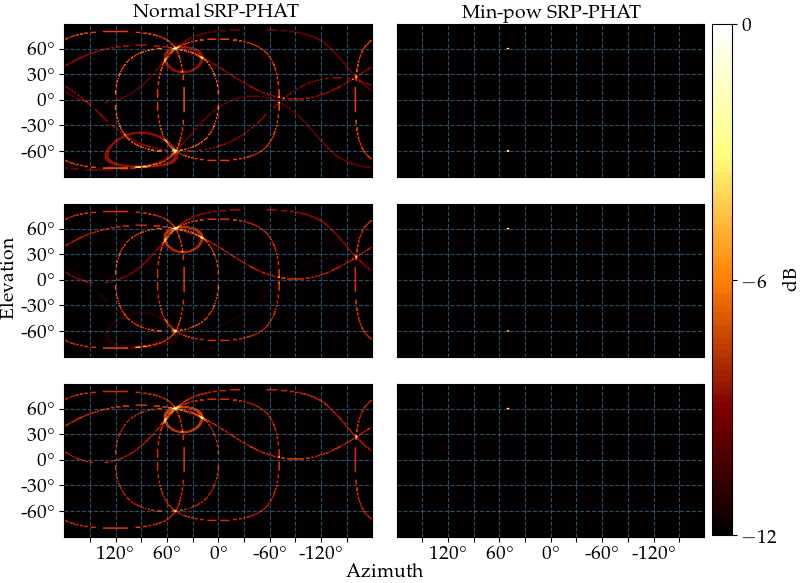
\includegraphics[width=\textwidth]{Figures/refSim.png}
\caption{Figures depict from top-to-bottom SRP-PHAT localization results with ground reflection coefficients (R) of 1, 0.6 and 0.1. The array has been tilted 30$\degree$ along the X-axis and 15$\degree$ along the Y-axis. This causes the ground image source to stop sharing cones with the real source and the correct relative power level between the image and real source is maintained for both normal SRP-PHAT and Min-pow SRP-PHAT}
\label{fig:4mic1srcRefTilt}
\end{figure}




\section{Filtering of the signal}

\begin{figure}[!ht]
    \centering
    \begin{subfigure}[b]{0.96\textwidth}
    \centering
    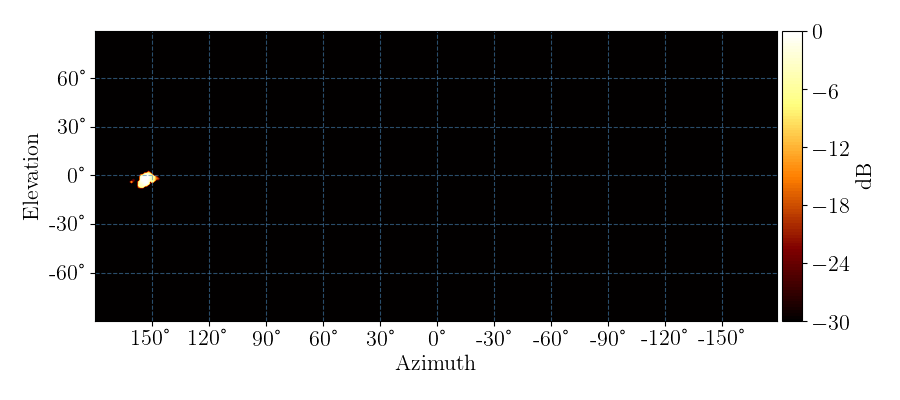
\includegraphics[width=0.8\textwidth]{Figures/chalkHi300MinPow.png}
\end{subfigure}
\vskip \baselineskip
\begin{subfigure}[b]{0.96\textwidth}
    \centering
    \includegraphics[width=0.8\textwidth]{Figures/chalklow300MinPow.png}
\end{subfigure}
\vskip \baselineskip
\begin{subfigure}[b]{0.96\textwidth}
    \centering
    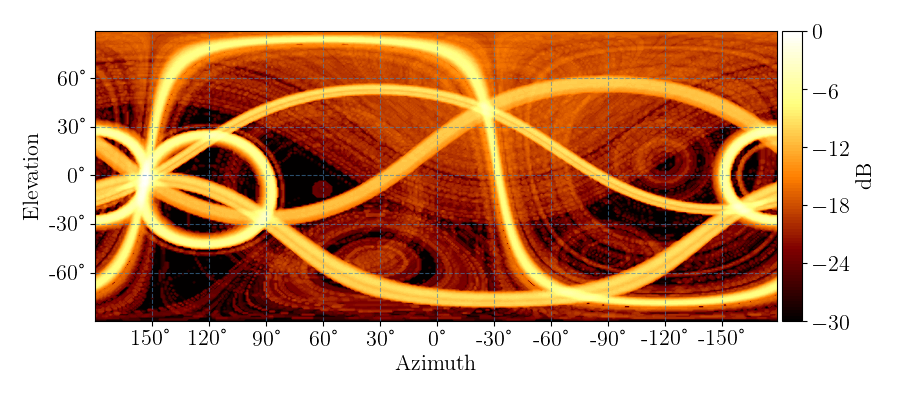
\includegraphics[width=0.8\textwidth]{Figures/chalkHi300Normal.png}
\end{subfigure}
\vskip \baselineskip
\begin{subfigure}[b]{0.96\textwidth}
    \centering
    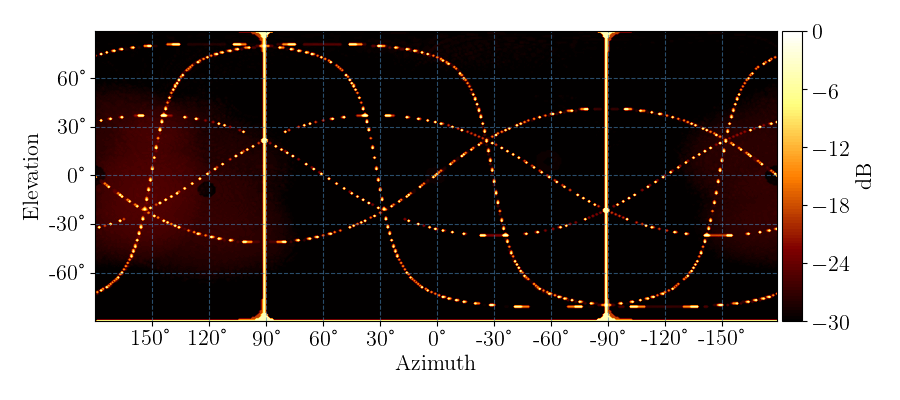
\includegraphics[width=0.8\textwidth]{Figures/chalkLow300Normal.png}
\end{subfigure}
\caption{Figures depict from top-to-bottom level SRP-PHAT localization results with high pass and low pass at 300Hz}
\label{fig:hilowfilter}
\end{figure}